\documentclass[12pt]{article}

%\usepackage{times}
%nips02e

\usepackage{spconf}
\usepackage{epsfig}
%\usepackage{psfig}
\usepackage{amsmath}
\usepackage[sort]{cite}
\usepackage{supertabular}
%\usepackage{dcolumn}
\usepackage{multirow}
\usepackage{rotating}
\usepackage{subfigure}
\usepackage{url}
\usepackage{bigstrut}
\usepackage{hhline}
%\usepackage{setspace}
%\usepackage{slashbox}
\usepackage[T1]{fontenc} % for bold small caps

\tolerance=1000
\hyphenpenalty=2000

%\textwidth 6.5in
%\textheight 9.0in
%\headheight 0.0in
%\headsep 0.0in
%\oddsidemargin 0.0in
%\evensidemargin 0.5in
\renewcommand{\topmargin}{-.25in} % AAA
\newcommand{\commented}[1]{}

%\global\boilerplate={}
%\global\copyrightetc{}

\newenvironment{packed_enum}{
\begin{enumerate}
  \setlength{\itemsep}{1pt}
  \setlength{\parskip}{0pt}
  \setlength{\parsep}{0pt}
}{\end{enumerate}}

\title{  AquaTux }
\name{David Biancolin, Adam Suban-Loewen, Victor Zhang, Ritchie Zhao}
\address{University of Toronto Mechatronics Design Association\\
email: mech.design@utoronto.ca }


\usepackage{comment}
% Un-comment one of the following two lines to turn pdf links on/off
%\includecomment{pdfrefs}
\excludecomment{pdfrefs}

\begin{pdfrefs}
\usepackage[ps2pdf]{hyperref}
% (See the hyperref package documentation for a list of supported drivers.)
\hypersetup{
    pdftitle={ AquaTux },
    pdfauthor={David Biancolin, Adam Suban-Loewen Victor Zhang, Ritchie Zhao},
    pdfsubject={AUVSI 2013},
    pdfkeywords={Mechatronics Design Association, AUV, submarine}
}
\end{pdfrefs}



%for subfigure
\renewcommand{\subfigcapskip}{0mm}
\renewcommand{\subfigtopskip}{0mm}
\renewcommand{\subfigbottomskip}{2mm}

\renewcommand{\topfraction}{0.999}     % max fraction of floats at top
\renewcommand{\bottomfraction}{0.99}        % max fraction of floats at bottom
\renewcommand{\floatpagefraction}{0.99}

\usepackage{amssymb}
\usepackage{fancyhdr}

\lhead{}
\chead{}
\rhead{}
\lfoot{}
\cfoot{Mechatronics Design Association -- University of Toronto}
\rfoot{\thepage}
\fancyheadoffset{0cm}
\renewcommand{\headsep}{10pt}   %AAAA
\renewcommand{\headrulewidth}{2pt}
\renewcommand{\footrulewidth}{2pt}
\renewcommand{\footskip}{0.5in}

\pagestyle{fancy}
\hyphenation{program-mable}
\hyphenation{pipe-lined}
\hyphenation{Chem-que}

\makeatletter
\renewcommand\maketitle{%
 \begin{minipage}[h]{.3\textwidth} 
   \centering 
   \includegraphics[width=2in]{fig/logo2} 
 \end{minipage}% 
 \begin{minipage}[h]{.7\textwidth} 
   \centering 
\vspace{.3in}
\Huge{AquaTux} \\
\vspace{.1in}
\large{ David~Biancolin, Adam~Suban-Loewen, Victor~Zhang, Ritchie~Zhao }\\
\normalsize{ University of Toronto Mechatronics Design Association\\
 email: mech.design@utoronto.ca }

 \end{minipage} 
\vspace{.3in}
\par}
\let\after@maketitle\@empty
\makeatother
\begin{document}

%%%%%%%%%%%%%%%%%%%%%%%%%%%%%%%%%%%%%%%%%%%%%%%%%%%%%%%%%%%%%%%%%%%%%%%%%%%%%%%%

\twocolumn[\maketitle]



\thispagestyle{fancy} 

\begin{abstract}
%In the context of the AUVSI and ONR's Xth International Autonomous
%Underwater Vehicle Competition, the team at the University of Toronto
%built an underwater vehicle.

AquaTux is the fourth entry of the University of Toronto Mechatronics
Design Association into the annual Autonomous Underwater Vehicle
Competition.  The vehicle is designed to autonomously complete
the set of tasks described in the mission\footnotemark[1].
It is equipped with an IMU, a depth sensor,
and two cameras that allow it to navigate in its environment.
This year's frame was reused from previous years.
We are proud to present new electronics, a new power system,
a new embedded system using an FPGA, and new software.

\end{abstract}


\vspace{-.1in}
\section{Introduction} 

The construction of the vehicle that our team will present at the
2013 Autonomous Underwater Vehicle (AUV) competition encompasses several new achievements. We explain the
context of our realization by first describing the main
objectives of the competition and how our team is organized.


\subsection{Overview of the Mission}

The objective of the competition is to build an autonomous underwater
vehicle to perform various tasks involving image recognition, and
passive sonar to
interact with its environment. For the vision-guided tasks, the vehicle must 
pass through a validation gate, hit buoys, follow pipes,
pass through set of pipes, drop an object
in a box, launch a projectile through a hexagonal target, and manipulating a wheel.
The sonar tasks consists of
grabbing an object on top of an acoustic pinger and surfacing above it.
The details of the required tasks for the vehicle are described in the
 mission specification on the AUVSI website\footnote[1]{http://www.auvsifoundation.org/foundation/competitions/robosub/}.
Through the design and testing phases, emphasis was placed on
performing a subset of these tasks well rather than attempting all tasks.

\subsection{The Team}
The team consists of twenty members that are divided into three subsystems: mechanical, electronics, and software. In order to maintain a high degree of integration throughout the project, members are encouraged to work in projects that span multiple subsystems. Our hardware is obtained through sponsorship and funding from our university (see Section~\ref{ack}). 

Figure~\ref{organi} illustrates the major components of the AUV
and the reader should refer to it often as we describe the innovative
aspects of those components in the following sections.


\begin{figure*}
\begin{center}
 \includegraphics[height=3.7in]{fig/arch.png}
\caption{Organization of the AUV modules and their connectivity.}\label{organi}
\end{center}
\end{figure*}



\vspace{-.1in}
\section{Frame design and construction}
The 2009 frame design underwent a complete revision based on our
experience from previous years.  Our past frame designs included
custom ordered molded or rapid prototyped parts intended to improve
the hydrodynamics of the hull.  After analyzing the conditions that
the vehicle would be subjected to, it was determined that the effects
of fluid dynamics were negligible in terms of functionality.  For this
reason, a ``design for manufacturing'' development methodology was
adopted: in efforts to minimize cost and machining time, the frame has been
designed to take advantage of commercial off-the-shelf parts as
well as capitalize on simple manufacturing processes.

\subsection{Design Considerations}
\label{fobjectives}
The design objectives in the 2009 frame were significantly more
ambitious as our team included more members adept in manufacturing.
The final concept was conceived such that it could be fabricated
without the need for outsourcing.

Below is the list of the desirable attributes for the frame that we set out to
obtain based on the experience gained from past frame designs:
\begin{packed_enum}
\item Minimize time required to access batteries and electronics;
\item Maximize modularity for easier transport and progressive revisions;
\item Optimize mass for transport, functionality and points;
\item Provide a secure removable internal rack for electronics to facilitate bench testing;
\item Obtain a a waterproof seal with a simple low tolerance assembly;
\item Create solid harness points and handles;
\item Facilitate movement through water and maximize battery life with
  a neutrally buoyant design;
\item Compensate for changes in mass distribution and motion
  calibration with adjustable thruster positions;
\item Design an attractive and professional looking vehicle.
\end{packed_enum}

\subsection{Frame Overview}
The AquaTux frame design can be divided into three
subsections: external frame, hull, and internal rack.  The goals based
on past experience described above suggested the need to
minimize the number of sealing surfaces and reduce the number of
waterproof connectors.  To achieve these objectives, a single enclosure
was created (the hull) to encapsulate everything except for the
markers to be dropped, the thrusters and the hydrophones.  These external components would be
connected to an exoskeleton type frame which allows for flexible
mounting arrangements.  Finally an internal rack was designed to hold
 all the electrical components including cameras and embedded computer.

\subsubsection{External Frame}
The external frame was designed with transportation and fabrication as
the primary constraints. This exoskeleton is made entirely of
commercial off-the-shelf
parts, $\frac{1}{2}$ inch PVC plumbing pipe and connectors.  The thruster positions
are fully adjustable since they are attached to individual pipes fixed
in place by standard gear clamps (Figure~\ref{adj}). The adjustability of the frame also
facilitates transportation as the entire structure can be collapsed to
fit a smaller envelope. 

\begin{figure}
\begin{center}
 \includegraphics[width=3in]{fig/dsc06455} 
% \includegraphics[width=3in]{fig/dsc06453} 
\vspace{.05in}
\hrule
\caption{Adjustable PVC tube exoskeleton frame.}\label{adj}
\end{center}
\end{figure}

In order to ensure a simple assembly method and utilize standard
connectors, the mechanism for picking up the briefcase was made of the
same material as the external frame.  It utilizes the fact that the
target is an open-walled structure and consists of a fork designed to
spear the case so that it can surface with the vehicle.

\subsubsection{Hull}
This year's hull design attempts to minimize the number of sealing
surfaces while maintaining usable space inside the vehicle.  In order
to seal the hull, a lid was made with a special simplified o-ring
groove (Figure~\ref{oring}). To avoid the need for precision milling or numerically
controlled machines, an oversized rectangular groove was cut.  The
corners were then drilled out and replaced with nylon dowels to
prevent the sharp corners from cutting into the o-ring.  This design
eliminated the need for specialized end mills or the need to mill
curved patterns in the lid. 

\begin{figure}
\begin{center}
 \includegraphics[width=3in]{fig/dsc06460.jpg} 
\vspace{.05in}
\hrule
\caption{O-ring displaced to show the grooves and nylon dowel.}\label{oring}
\end{center}
\end{figure}

Past experience suggested the need for a quicker method to access the
internal components of the hull.  Quick-release latches 
(Figure~\ref{quick}), were
used to replace nuts and bolts which take significantly more time to
release.  These latches use a cam mechanism to clamp the lid to
metallic bars and subsequently compress the o-ring, creating a water-tight seal.

\begin{figure}
\begin{center}
 \includegraphics[width=1.34in]{fig/dsc06462} 
\vspace{.05in}
\hrule
\caption{Quick release cover mechanism.}\label{quick}
\end{center}
\end{figure}

An endplate was designed to provide a single replaceable surface to accept all the connectors between the interior and exterior of the vehicle.  This endplate is sealed with a groove similar to that of the lid and is attached with self sealing screws from APM Hexseal.  The waterproof connectors which pass through the endplate lead to two master-disconnects which allow for quick and easy installation of the internal rack (Figure~\ref{endplate}).
The waterproof connectors chosen are 8-pin Neoprene molded connectors
from Impulse Enterprise.  These connect the thrusters as well as the
wireless tether and provide maximal flexibility due to their pin count
as well as small profile.  
The pressure readings for the AUV are also gathered  through the
endplate. In order to sense depth, a MPX4115 pressure transducer is
coupled to a segment of PVC tubing connected to a compression nut on
the endplate.  The depth of the vehicle corresponds to the pressure of
the air trapped in the PVC tubing.
  The hull is fabricated from
$\frac{1}{8}$ inch thick polycarbonate sheets, with waterproof epoxy bonding
the joints together.  To strengthen the bonds, aluminum angle brackets
were added to the edges to increase the bonding area of the epoxy. The thin, clear polycarbonate walls of the hull allow subsystems such as the cameras, marker droppers (section~\ref{mdroppers}) and trigger for the torpedo to operate from within the vessel.

\begin{figure}
\begin{center}
\subfigure[Endplate showing waterproof connectors.]{ \includegraphics[width=3in]{fig/dsc06464} }
\subfigure[Master disconnects for the waterproof connectors on the
inside of the vehicle.]{ \includegraphics[width=3in]{fig/dsc06465} }
\vspace{.05in}
\hrule
\caption{Connection system to the outside of the vehicle.}\label{endplate}
\end{center}
\end{figure}

\subsubsection{Internal Rack}
In addition to remedying problems with our previous frames, we
endeavored to produce a frame that could be reconfigured and usable in
future years.  The concept for the internal rack (Figure~\ref{rack})
consists of base plates that accepts stacks of electronics.  These
plates can be removed as a single unit which facilitates wiring, and
bench testing.  Due to the buoyancy of the hull, stainless steel bars
were used to add weight to the vehicle (Figure~\ref{rack}).  These weights act as a method of balancing the
vessel and allow the electrical components to be reconfigured for
years to come.  The internal rack does not rest directly on the floor
of the hull.  In case of a leak, water would collect in the space
below the electrical components and be detected with leak sensors
prior to any damage.


\begin{figure}
\begin{center}
 \includegraphics[width=3in]{fig/dsc06466} 
\vspace{.05in}
\hrule
\caption{Inside rack holding the electronics and the stainless steel weights.}\label{rack}
\end{center}
\end{figure}


\section{The Marker Dropper}
\label{mdroppers}

The thin walls of the hull facilitate the operation of a simple marker dropper system which
can be centered around the downward facing camera.  Two ferrous
markers are placed on the exterior of the vessel and held in place by
a magnetic attraction to two rare earth magnets located on the inside
of the hull.  The magnets are connected to individual stepper motors
which retract the magnets from the wall of the hull (Figure~\ref{md2}).  The increased
distance between the magnets and the markers causes a reduction in
magnetic field strength allowing the markers to drop freely from the
vehicle.

\begin{figure}
\begin{center}
 \includegraphics[width=3in]{fig/dsc06468} 
\vspace{.05in}
\hrule
\caption{Two marker-droppers: from top to bottom, a stepper motor
  retracts a magnet from the surface of the hull (bottom in the figure).}\label{md2}
\end{center}
\end{figure}

\section{The Torpedo Launcher}
\label{torpedo}
\vspace{-.1in}
One of the primary goals of this year's entry into the AUV Competition
was to minimize the number of connections that pass through the
endplate of the hull.  The resulting design for a torpedo launcher was
an external system that was activated by a magnetic switch.  This
concept allowed us to mimic the marker dropper design to activate the
torpedo.  The external system  contains only a few simple parts; a
power supply (9V battery), a solenoid valve, a magnetic switch, a
compressed gas cylinder and a projectile. As the magnet in the hull
is retracted from the hull, the magnetic switch is
triggered.  The switch  then triggers the solenoid valve allowing
compressed gas to fire the torpedo.

The controls for the above mentioned systems are described in the
following sections.

\vspace{-.1in}
%\section{Electrical aspects}

\section{Electronics}
Our electronics were designed to handle all low-level tasks that are
required to move AquaTux, acquire sensor data from the IMU and depth sensors. 
The main goal of the electronics is to allow the AUV to be driven with only
high-level heading and depth commands. The electronics are responsible for
executing the commands and controlling their results (e.g. depth or
heading) in a ``black box'' fashion. The electronics are managed by the embedded
system described in the next section, giving access to each electronic peripheral.

Aquatux's electronics are arranged in two stacks of PCBs, one dedicated to power 
distribution and management, and the ``main stack'', which breaks out the on board 
FPGA's I/Os to any number of children.

\subsection{Main Stack}
At the heart of Aquatux's electronic subsystem is a Terasic DE0-Nano, a small 
form-factor FPGA development board, containing an Altera Cyclone IV FPGA. The 
DE0 mates directly to the ``Interface Board'' which breaks out all of the 
available I/0s to a 120 pin board to board connector (Figure~\ref{mstack}). Any number of new PCBs 
can be mated, by providing the mating male and female connectors. These 
connectors form a wide bus between the FPGA and the mating boards, which when 
coupled with the reconfigurability of an FPGA, makes it very easy to incorporate 
new PCBs without having to physically rewire parts of the submarine -- a Quartus 
recompile is all that's required. The interface board also connects to the IMU, 
a VectorNav VN-100 Rugged, which performs its own sensor signal processing to 
output attitude data to the FPGA.

\begin{figure}
\begin{center}
 \includegraphics[width=3in]{fig/main_stack.png} %1.34
\vspace{.05in}
\hrule
\caption{The main stack connector. Top, the interface board and DE0 nano. Below, two 6 channel motor drivers.}\label{mstack}
\end{center}
\end{figure}

\subsection{Motor Board}

The motor boards are used to control the Seabotix BTD150 Thrusters used on AquaTux 
and other actuators internal to the submarine. Each motor board (Figure~\ref{motorb}) consists of 6 NMOS 
high-side half bridges driven by Linear Technologies LT1660 half-bridge drivers. 
Each half bridge has a sister with which it can be used a full bridge, by soldering 
the output connector in the correct position. Complementary PWM inputs to each driver 
can be sourced from one of three sets of I/Os provided via the main stack connector, 
allowing a multiplicity of boards to be mated to the stack. Presently, two of three 
boards are used, providing the five full bridges required to drive Aquatux's motors. 
The final board is provision to drive internal peripherals such as marker droppers in 
future competitions.

\begin{figure}
\begin{center}
 \includegraphics[width=3in]{fig/motor_board.png} %1.34
\vspace{.05in}
\hrule
\caption{A motor board, configured with 3 full bridges.}\label{motorb}
\end{center}
\end{figure}

\subsection{Power Distribution}
Power for Aquatux's electronic systems, excluding the netbook, is provided by 
two 24V NiMH battery packs. The power distribution board switches the battery 
voltage with a relay, which is controlled by the FPGA's soft-processor. 
Throwing the kill switch (by removing the velcroed handle on the side of the 
hull) opens a reed switch which breaks the relay's coil current. Three DC/DC 
converters (3.3V, 5V, 12V) source from this voltage, and form a stack of PCBs 
with the power management board above them. LC output filters on power management 
board remove switching harmonics, before breaking out the rail voltages to the 
submarine through a series of copper bus-bars. Four pairs of analog comparators 
alert the FPGA when any of the rails over or under-volts by 5 percent of their nominal 
voltage. As a final baseline precaution, breakers have been inserted between the 
batteries and relay, and between the power management board and bus-bars for each rail.

\subsection{Power Source}
The NiMH battery packs were custom designed by our team: each pack is
composed of 20 SY136T Sanyo nickel metal hydride batteries. All
batteries are connected in series to form a 24V nominal battery pack
with a capacity of 4100mAh. Temperature sensors embedded in each pack allow 
the FPGA to kill the sub if any one pack overheats.

\vspace{-.1in}
\section{Embedded System}

The embedded system was designed to link the submarine's computer with all
electronic peripherals, with a high-level interface to access groups of peripherals.
The embedded system consists of a DE0-Nano FPGA, synthesizing custom circuitry to
communicate with each peripheral and a soft processor to communicate with the computer. The FPGA was chosen
for its quantity of general-purpose I/O pins, allowing it to manage all electronic peripherals,
and its compact size of 3x2 inches. The FPGA is the only programmable element in the submarine
besides the computer, reducing the amount of communication between programmable elements.

\subsection{FPGA Soft Processor}

The FPGA Soft Processor exposes high-level commands to the computer to access each group
of electronic peripherals.
The IMU and depth sensor provide attitude readings and are used by the PID controllers and the
computer interface. Power management continually monitors each
voltage rail, and will power off the submarine if any voltage is invalid.
The five motor drivers are controlled together by the soft processor's yaw, pitch, roll,
and depth PID controllers. The computer interface can set target
speed, yaw, and depth, which are inputs to the PID controllers. Speed is implemented as an offset
because the submarine does not have velocity measurement. The PID controllers are implemented on the
soft processor because they need immediate access to the motor drivers and attitude readings.
The high-level commands are
text-based, allowing manual control to test each peripheral individually.
Future plans for sonar processing will be implemented on the FPGA, using the soft processor and
built-in DSP elements.

\subsection{FPGA Hardware}

The FPGA also synthesizes custom hardware to communicate with peripherals through general-purpose pins.
This flexibility can support any protocol to communicate with peripherals, including SPI and UART.
Each peripheral protocol is a separate module, memory-mapped to the soft processor across Altera's
Avalon Bus. The DE0-Nano has 85 general-purpose pins for digital inputs and 8 ADC inputs.
The depth sensor is an analog peripheral, and all other peripherals communicate digitally.
The hardware and soft processor run at 50 MHz.

\vspace{-.1in}
\section{Software}

The submarine's software is aware of the competition objectives, and performs computer vision to
command the submarine to move through the embedded system.
The software is organized so that it is easy to test the core vision and control systems with different
sources of video input and to command the submarine or the simulator to move.
The software also includes a graphical simulator that we can use to test our vision and control algorithms.

\subsection{Software Organization}
\label{gui}


\begin{figure}
\begin{center}
 \includegraphics[height=1.9in]{fig/modules.png}
\caption{Software module organization.}\label{modules}
\end{center}
\end{figure}


\begin{figure}
\begin{center}
 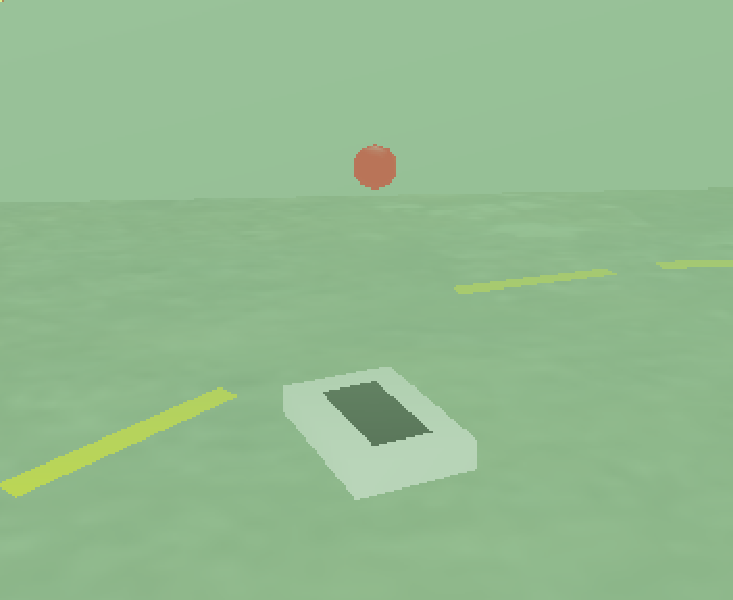
\includegraphics[height=1.9in]{fig/sim.png}
\caption{Example image from the simulator showing pipe segments and the buoys
         in turbid water.}\label{sim}
\end{center}
\end{figure}

The software is broken down into 3
components (Figure~\ref{modules}): (i) the video input;
(ii) the mission software gives physical commands to move the sub;
and (iii) the environment that reacts to the physical commands.
The video input can come from the submarine's webcams, pre-recorded video,
or the simulator (Figure~\ref{sim}). The mission software can be the autonomous
algorithms that drive the submarine or a manually controlled user interface.
The environment that reacts to physical commands can be the submarine or the
simulator. The different permutations to hook up the software components
solely created to test and debug the vision
algorithms when AquaTux is not functioning autonomously.
These software interfaces help ensure the software to test the submarine
resembles the autonomous functionality as much as possible.
The manual user interface allows us to act as a passive observer,
constantly requesting the state of the vehicle,
or as a controller sending commands to the AUV.

\subsection{Simulator}
The simulator is a piece of software written in C++ using the OpenGL library. Its purpose is to simulate the competition grounds so the software and vision algorithms can be tested with greater ease. The simulator was extremely useful, as using a pool is both expensive and time consuming.

The simulator contains a physical model of each obstacle in the competition,  as well as a method to track the locations of the two cameras on the sub. OpenGL calls are then used to draw the images that would be seen by the cameras, which are then extracted to the image processing algorithms (Figure~\ref{sim} shows an image that would be seen by the forward camera).
The simulator can accept commands to move the camera viewpoint, so that we can properly simulate video feedback when the submarine is commanded to move.

\subsection{Software Control}
Our control algorithms are run the submarine runs autonomously. The entire mission is broken down into tasks, such as the gate or buoy task,
which are implemented in separate modules. The control code queries the vision system for circles, lines or rectangles, and translates the
vision result into a movement command. While the submarine is reacting to a movement command, the video input is ignored to prevent
overshooting or oscillating the target.
Each control task can be tested separately.

\section{Vision}
The machine vision system is defined as all software and hardware which converts images (the input to the system) into numerical data (the output). This data refers primarily to the existence, position, orientation, and color of various objects in the image, such as the starting gate or a colored buoy. This information is handed off to the rest of the software, which acts on it to determine the correct course of action for the submarine. Because the internal representation of an image is simply a large matrix of numbers, the vision system's job can be thought of as filtering this large volume of mostly extraneous data to a few pieces of useful data, which the control system can then analyze.

\subsection{Vision Hardware}
The hardware for the vision subsystem consists of two cameras and a small netbook. Both cameras are Logitech Webcam 9000 Pro webcams, one of which points forward, and the other of which points down. These cameras were chosen for their price (about \$50 each) and the availability ofLinux driver support. While the cameras are not specifically designed for underwater or low light conditions, they have worked quite well in our pool testing. The netbook used is an HP Atom netbook. This model was chosen for its small size and low cost.

\subsection{Vision Software}
All of our image processing code is written in C++, using the OpenCV library. A large number of algorithms were tried and discarded during the development of our final flow.  Due to the scope of this document only the final algorithms used will be described.

The image processing flow can be broken up into three distinct parts: image segmentation (separating a 3-channel image into 1-channel pieces based primarily on color), object recognition (classification of each segment as background or target) and property calculation (deriving the object's properties such as location or color). The algorithm used for each step is distinct and will be discussed below.

Image segmentation is performed using OpenCV's implementation of the Watershed algorithm. The algorithm works iteratively from a collection of segmented pixels (seeds) and at each step associates the most similar pixel adjacent to a segmented pixel with that segment. It returns a grayscale image, with different gray levels corresponding to different segments. Each seed pixel has a value associated and two seeds of the same value will contribute to a single segment.

The performance of the Watershed algorithm is heavily dependent on the quality of the seeding. Optimally we want at least one seed for each different object in the image and at least one seed for the background. A single object should not have two different valued seeds, as this will cause two segments to emerge. To seed the algorithm, we take a random sample of pixels from the source image, and run K-Means clustering to cluster the samples based on color similarity. The results of the clustering is a minimum collection of pixels which are representative of the color space of the image. The clustering results used to assign values to the seeds - similarly colored seeds will get the same values (Figures~\ref{seed} and \ref{segment}).

\begin{figure}
\begin{center}
 \includegraphics[height=1.9in]{fig/seed_image.jpg}
\caption{Example image at a test pool, with seed locations overlayed.}\label{seed}
\end{center}
\end{figure}


\begin{figure}
\begin{center}
 \includegraphics[height=1.9in]{fig/segmented_image.jpg}
\caption{The test image segmented.}\label{segment}
\end{center}
\end{figure}

Object recognition is made simple due to the fact that only circles and rectangles need to be recognized for the tasks we are aiming to do. OpenCV can find the minimum enclosing circle and (rotated) box for any segment, and a simple comparison of area, perimeter, and various symmetry properties can be performed to check if the segment is similar to its enclosing shape. For example, a the minimum enclosing circle of a non-circular segment will leave large amounts of blank space, and will therefore have a very different area compared to the segment.

Property calculation is done on a target-by-target basis. For most targets (the buoy, for example), it is  sufficient to know the position and characteristic dimension in pixel space. We can then use these numbers, along with the camera's field-of-view and the physical length to calculate the position and range of the object in real space. For the pipes at the bottom of the pool, the position angle is also needed. All of the pixle properties are easily extracted from the enclosing shape derived by OpenCV. To identify an object's color, we convert the BGR color of the object into HSV, which is more robust against changes in brightness, and use the resulting hue value to determine the color of the object.

Finally, in order for the vision code to return stable results and be robust against noise, we store the objects identified in the current frame begin processed as well as a number of frames prior. We use this to average and filter the numerical information from multiple frames. This allows us some room for error - a single frame with poor segmentation or a stray object will not destroy the system's performance.

\vspace{-.1in}
\section{Conclusions} 
\vspace{-.03in}

This year's team took on the challenge of building all of Aquatux's electronics
and software within the existing frame. This AUV is composed of a Netbook that
is linked to a single FPGA that drives the electronic peripherals.
The Netbook runs mission-aware vision software, which uses the OpenCV library.
Circuit board fabrication, plastic machining, embedded programming,
and software engineering are some
of the skills that many of our members were able to acquire. More
rational design techniques and project management skills are also
derived from the our previous competitions and they had a significant
effect on maximizing the productivity of all the man-hours contributed
to the project.


\vspace{-.1in}
\section{Acknowledgments}
\label{ack}
\vspace{-.03in}

We would like to thank the staff of the University of Toronto for
supporting our project.

We would also like to thank all our sponsors who have helped make this
project possible: The University of Toronto Engineering Alumni
Association, The Edward S. Rogers Department of Electrical and
Computer Engineering, The Division of Engineering Science, the
University of Toronto Engineering Society, and Altera.

%\vspace{-.08in}
%\small
%\bibliographystyle{IEEEtran}
%\bibliography{IEEEabrv,paper}


\end{document}
